\chapter{WebRTC Trust and Security Model}
\label{webrtcmodel}

\begin{quote}
\textit{
In this chapter, we propose a trust and security model of a WebRTC session.
Our model integrates into a single metric the security parameters used to establish the session, the media encryption parameters, and user's trust in actors of the WebRTC session.
The first objective of our model is to answer RQ1: ``What are the risks for the user of a WebRTC session and which abstractions can we use to show these risks to the user''?
In particular, we intend our model to help advanced users: \ie users that would be susceptible to look under the hood, but without expertise in web security.
We first present our methodology to build our model in Section~\ref{sec:methodologyModel}, and then detail our WebRTC trust and security model in Section~\ref{sec:webrtcmodel}.
The model evaluates security with regards to the risk presented on the confidentiality and integrity of the communication and shows which trust relations must be valid in order for the security level to be trusted too. 
In order to validate our approach, we present in Section~\ref{sec:validationModel} a preliminary study on the understanding of our model by advanced users.
This study is based on a survey containing a dynamic implementation of our model which allows modifying the trust and security parameters.
}
\end{quote}

\begin{figure}[H]
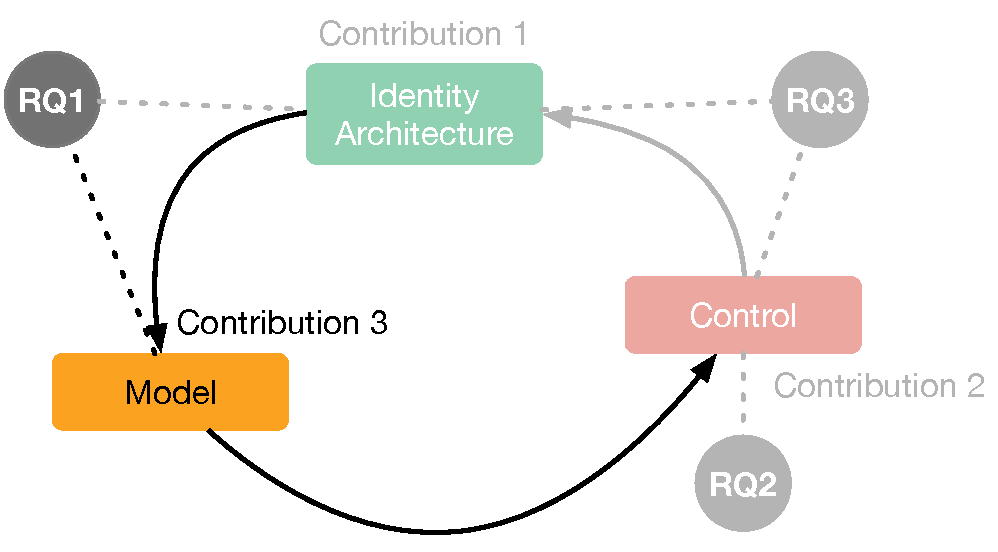
\includegraphics[scale=.5]{images/contrib3}
\caption{Overview of our Contributions: Modelling the WebRTC Trust and Security.}
\label{contrib3}
\end{figure}

\clearpage

\glsresetall
\section{Methodology}
\label{sec:methodologyModel}

As we stated in our Introduction chapter:

\begin{quote}
\textit{``Our intuition is that users should be given more information and control over the security and trust level of their communications. This is our global objective. For this to be possible, we need to build a model that could represent the communication setup, the different channels, protocols, and the actors in operation. This model would allow us to forge a single metric characterising the risk of using the communication system, \ie the trust and security level.''}
\end{quote}

Several methods and models have already been proposed to model the security or trust of a communication system.
We reported in our state of the art (see Section~\ref{sec:sota2012+}) that Beltran~\etal\cite{beltran2014user} propose a trust model of the WebRTC identity architecture in a single \gls{cs} scenario. 
Building on this work, Javed~\etal\cite{javed2016browser,javed2016br2br,javed2017trustcall} work on reputational trust models for WebRTC representing trust, distrust, and mistrust\footnote{This idea of representing trust, distrust, and uncertainty was first defined by Josang\cite{josang1997artificial} as subjective logic.}.
In their last proposed model~\cite{javed2017trustcall}, the user's reputation is the weighted sum of the user's behavioural trust and a measure of its authenticity as presented in Figure~\ref{fig:javedModel}.
They explicitly refer to trust visualisation and help to users' decision as possible uses of their trust model.
However, their approach does not completely fit our objective of a security and trust model.
Indeed, security considerations in their model are quite limited and only consider the authenticity of the other peer, a remark we also made on their earlier~\cite{javed2016br2br} in our state of the art.
Furthermore, in this model the authenticity of a peer is actually a reputation score rather than a measure of actual authentication.
While it would be acceptable to aggregate authentication score from multiple recommenders, \ie identity providers, the model does not discuss the binding of these identity assertions with the actual WebRTC session.
It seems that authenticity is here used with a different meaning as the one we use in this thesis.

\begin{figure}[tb]
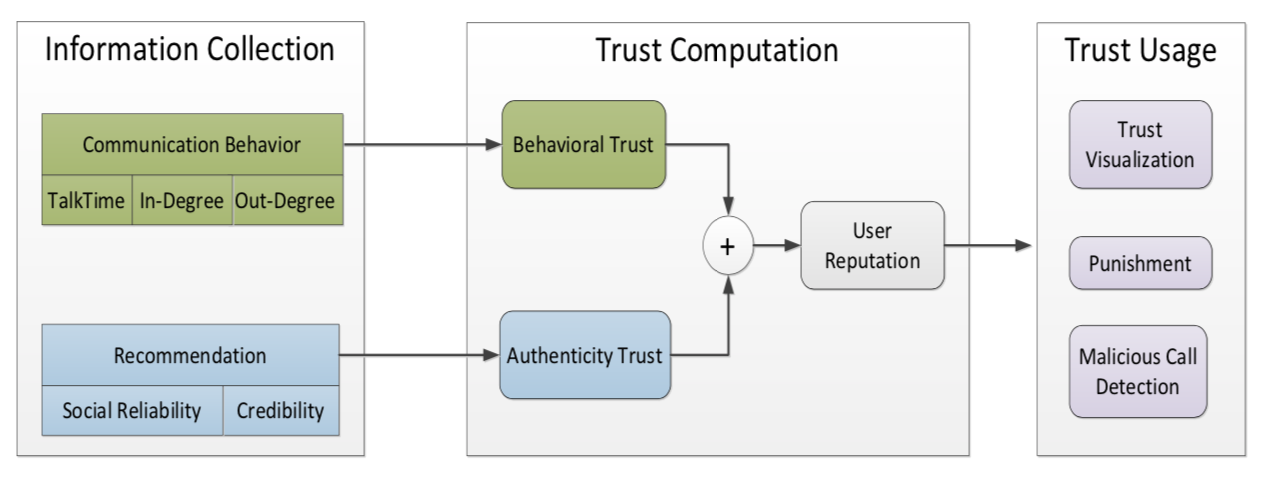
\includegraphics[scale=.6]{images/trustCall}
\caption{Javed \etal TrustCall architecture~\cite{javed2017trustcall}.}
\label{fig:javedModel}
\end{figure}

We also reported on a model by Alia \etal\cite{alia2010putting} which propose a component-based adaptation model to manage the trade-offs between \gls{qos} and Security.
They model an adaptable \gls{voip} system as a composition of components each providing different \gls{qos} and security properties.
A utility function aggregating \gls{qos} and security dimensions, shown in Figure~\ref{fig:utilityFunction2}, allows discriminating between different configurations.
Considered dimensions are the latency and video scheme quality for \gls{qos} and the confidentiality, anonymity, and authentication for security.
Their model also uses user's preferences as weight in the utility function and risk context as minimal required value for each security dimension.
While we do not consider \gls{qos} in our approach, we pursue a similar long-term objective of managing the security level.
However, in our view, this model also shows a limited security model.
For instance, the confidentiality function (presented in Table~\ref{tab:aliaFunction}) only considers security over the media path.
Other parameters of the session setup, such as the security of the signalling path or the authenticity of the other peer, would have a major impact on the confidentiality level but are not considered in this function.
We also note that the value attributed to the utility functions seems arbitrarily defined.
This is, for instance, the case with the confidentiality function shown in Table~\ref{tab:aliaFunction} which follows a linear increase.

\begin{figure}[tb]
\begin{center}
$U = W^{lat}.F(lat) +  W^{qua}.F(qua) + W^{conf}.F(conf) +$\\

$ W^{anon}.F(anon) + W^{auth}.F(auth)$
\end{center}
\caption[Alia~\etal\cite{alia2010putting} Overall Utility Function]{Overall utility function~\cite{alia2010putting} where $F(k)$ are the utility functions and $W^k$ user preference weights for dimensions $k$ as latency, video scheme quality, confidentiality, anonymity, and authentication.}
\label{fig:utilityFunction2}
\end{figure}

\begin{table}[tb]
\begin{tabular}{{@{}lccc@{}}}\toprule\toprule
  Encryption Algorithm& Key Length & $F(conf)$ & Performance Overhead \\\midrule
  DES & 56 & 0.2 & 0.2 \\
  AES & 128 & 0.3 & 0.3 \\
  Blowfish & 128 & 0.4 & 0.4 \\
  Blowfish & 448 & 0.5 & 0.5 \\
  \bottomrule
  \hline
\end{tabular}
\caption[Alia~\etal\cite{alia2010putting} Confidentiality Utility Function]{Confidentiality utility function $F(conf)$ and performance overheads from Alia~\etal\cite{alia2010putting}.}
\label{tab:aliaFunction}
\end{table}

Another methodology for modelling security of systems is to build attack trees. 
These models are an analytical approach towards identifying possible attack vectors.
Our researches on the state of the art (see Section~\ref{sec:sota2012+}) and specific research on ``WebRTC attack tree'' did not reveal any publication of a WebRTC attack tree. 
While the STREWS D1.2 document~\cite{bos2014case} and STREWS D1.1 document~\cite{de2013web} refer to an attack tree as a step of their methodology to map threats to WebRTC assets, no such tree has been published in these documents.

\begin{figure}[tb]
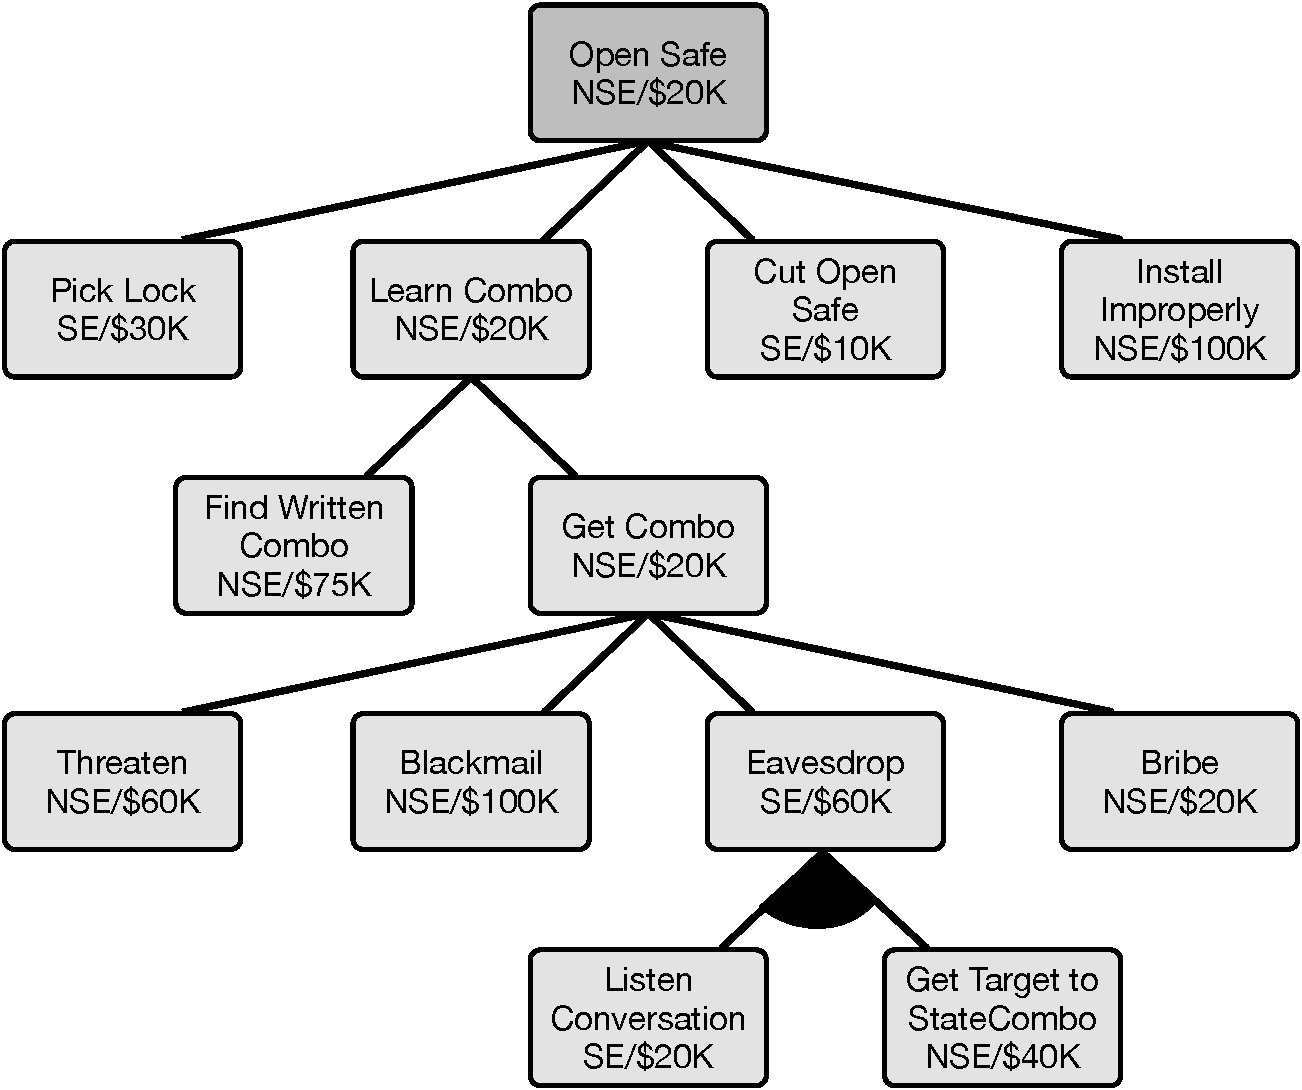
\includegraphics[scale=.45]{images/schneier}
\caption[Attack Tree Example]{Cheapest attack requiring no special equipment against a safe~\cite{schneier1999attack}. The black ark denotes an \textit{AND} relation, empty arks denote \textit{OR} relations.}
\label{fig:schneierModel}
\end{figure}

As described by Bruce Schneier~\cite{schneier1999attack}, creating an attack tree is an iterative process starting with the identification of possible attack goals.
Then for each goal, possible attacks are added to the tree which will, in turn, require the completion of new attack goals for the attacker.
By default, the relation between an attack goal and its sub-goals is defined as an \textit{OR} relation, \ie at least one of the subgoal must be accomplished for the parent goal to succeed.
Some other relations can be defined with an \textit{AND} operator.
In these cases, each subgoal must be accomplished for the parent goal to succeed.
Various values can be further derived from an attack tree by assigned value to leaf or nodes of the tree.
For instance, these values may be the cost, difficulty, or conditions required to accomplish an attack.
This allows for instance to compute the cheapest possible attacks requiring no special equipment, as in Figure~\ref{fig:schneierModel}.
This decomposition process is iterated as necessary until no more attacks are found.

To build our trust and security model we follow an iterative decomposition process, in a similar way to attack tree decomposition.
However, the intent of the model is to inform the user of the security of its communication setup. 
It needs to be instantiated with measurable security properties.
We thus stop the decomposition of security properties at measurable elements or where policies can be defined.

In Section~\ref{sec_sdp} we discussed which actor would be best suited to provide trusted identity recommendation and negotiation capabilities.
We concluded that between the \gls{idp}, \gls{cs}, and Browser, no actors appeared clearly more suited to evaluate and negotiate over the other party authentication.
The other peer authentication is only a subset of the security parameters that need to be monitored, but in our opinion, a similar reasoning applies to the overall WebRTC security parameters.
We thus suppose that the browser is instantiating the trust and security model and consider only elements that can be observed by the browser. 

We previously cited J{\o}sang and Presti defining trust as ``the extent to which one party is willing to depend on something or somebody in a given situation with a feeling of relative security, even though negative consequences are possible''~\cite{josang2004analysing}.
To build our model, we start from a high-level trust property node: the trust of the user Alice in the confidentiality of her communication.
We then iteratively decompose nodes into their dependencies which are either other high-level trust, security properties or trust relations with other actors.
We note trust as $T_X(Y)$ where $X$ is the truster and $Y$ is a trusted property (for high-level trust properties) or a trusted actor (for trust relations).
The decomposition process is carried on until a satisfying level of details is reached.
Dependencies in attack trees are represented either using an \textit{OR} or \textit{AND} relations as explained previously and we use the same logic in our decomposition.
Note that as we model security rather than attacks, for the same scenario the signification of operators is the reciprocal of the equivalent attack tree.
For instance, if each attack subgoals must be accomplished as represented by an \textit{AND} operator, our security model would use the \textit{OR} operator meaning that at least one defence dependency must hold.
We both model our security and trust tree in graphical and outline form. 
Graphically we use the same representation as in Figure~\ref{fig:schneierModel} while in outline form we use the postfix decomposition operators $\otimes$ and $\oplus$ respectively for \textit{AND} and \textit{OR}.

As we model the trust and security from an end-user point of view, not all security properties are visible and leafs of this model are thus either security properties or trust relations.
For instance, the secure connection between both $CS_A$ and $CS_B$ is not visible by Alice.
Thus Alice can monitor her secure connection with $CS_A$ but must trust $CS_A$ for the rest of the signalling path.
In order to offer an alternative omniscient model, we continue the decomposition process from terminal trust relations to observe the trust and security model beyond.
We define terminal trust relations as being transitive trust relations from trust in an actor to trust in a security context. 
Graphically, such transitive trust relations are represented as dashed lines while in outline form we use a grey font to represent this omniscient model and $\rightarrow$ as the transitive operator.


%Such dependencies are either other trust relations or security properties that can be evaluated.
%Additionally, a trust relationship is also dependent on a particular context, as we described in Section~\ref{sec:trustintro}.
%Explain what we call context.
%Thus a trust relationship may be valid for a context, but not for another.
%If a trust relations is decomposed into several other trust relations, these are not necessarily all from the same context.
%Said otherwise, trust contexts can also be decomposed into other trust contexts and relations.
%As an example, trust is often understood as the reliability of a trustee.
%But in order to consider the reliability of a peer, it is first necessary to ensure that it is correctly authenticated.
%Similarly, as we mention in Section~\ref{}, the authentication, or the identity context, is dependent on adequate security configurations.
%We thus identify dependencies between reliability -> identity -> security as represented in Figure~\ref{}.


\section{Building the WebRTC Trust and Security Model}
\label{sec:webrtcmodel}
In this section, we model the trust of Alice in the confidentiality of her WebRTC session with Bob.
In this scenario, Alice and Bob setup their WebRTC connection each on a different communication service, respectively $CS_A$ and $CS_B$ and both use an Identity Provider, respectively $IdP_A$ and $IdP_B$\footnote{The session architecture is similar to the one presented in Figure~\ref{fig:webrtcDeployId}.}.
We do not consider attacks conducted by the web application such as interception or redirection attacks.
Similarly, we do not consider User-Agent and Operating System trust relationships with users in our model. 
As the WebRTC specification consider the User-Agent to be the Trusted Computing Base, we adopt the same point of view. 
Clearly, if the Trusted Computing Base or lower stack software and hardware are corrupted, the whole communication is at risk.

\subsection{Session Confidentiality}
In order to trust that the communication setup ensures the confidentiality of the communication, Alice must have trust in the two following properties:
\begin{itemize}
\item The other peer's authenticity, \ie that Bob is who he claims to be and that no man-in-the-middle is present on the wire.
\item The confidentiality of the peer-to-peer communication between Alice and Bob, \ie that an attacker cannot decrypt the media stream.
\end{itemize}

Attacks against both these properties are described in the STREWS D1.2 document~\cite{bos2014case}.
As both properties must hold, the trust of Alice in the confidentiality of her WebRTC session is equal to the minimum trust in each of these properties.
We represent this relation graphically as in Figure~\ref{fig:df_webrtc} and in outline form in Definition~\ref{def:df_webrtc}.
Without explicit authentication, the other peer's authenticity depends on actors operating on the signalling path.

\begin{figure}[tb]
\begin{subfigure}[b]{0.45\textwidth}
\centering
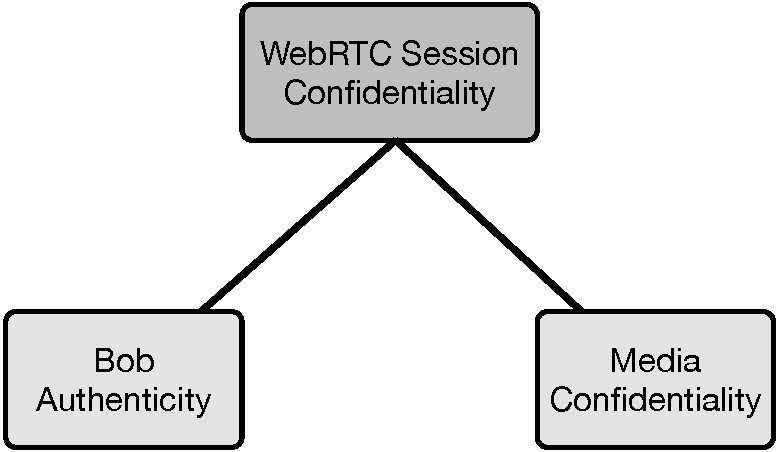
\includegraphics[scale=.5]{images/df_webrtc}
\caption{Graphical representation.}
\label{fig:df_webrtc}
\end{subfigure}
~
\begin{subfigure}[b]{0.45\textwidth}
\begin{equation*}
\begin{split}
&T_A(conf(Session_{A,B,M})) \quad\otimes \\
&    \quad T_A(auth(B))\\
&    \quad T_A(conf(M))
\end{split}
\end{equation*}
\caption{Outline form.}
\label{def:df_webrtc}
\end{subfigure}

\caption{Alice's trust in the confidentiality of her WebRTC session.}
\end{figure}


\subsection{Signalling Path Security}
Alice relies on the signalling path to establish a peer-to-peer session with Bob.
She must trust both communication services, $CS_A$ and $CS_B$, to correctly route call offers and answers to Bob.
The risk faced is that a man-in-the-middle may be set up, either by one of the communication service or by an external attacker leveraging an insecure signalling path.
We decompose trust in the signalling path as in Figure~\ref{fig:df_signalling}.

To trust the signalling from Alice to Bob, Alice has to trust the security of the first link, \ie the \gls{tls} connection between her and $CS_A$, as well as the remaining of the signalling path from $CS_A$ to Bob.
To this end, Alice has to trust $CS_A$ to behave honestly and securely.
The rest of the signalling process is however invisible from Alice's point of view and could not be instantiated.
Nonetheless, we represent it in our model for later discussions using dashed lines in graphical form and grey font in outline form.
In the simplest scenario, two users setup their WebRTC connection using a single communication service operating in silo.
With multiple \gls{cs} as we consider in this case, the user chooses its own service but may not know through which service the call signalling transits.
Communication services may be federated around a unique signalling federation or operate using a circle of trust model.
For Alice, its trust relationship with the other party service, $CS_B$, transits through its own service $CS_A$.
Thus we then consider $CS_A$ trust in the remaining of the signalling path from $CS_B$ to Bob.
Similarly to Alice's trust, $CS_A$ has to trust $CS_B$ to behave honestly and that $CS_B$ uses a secure connection to Bob.
$CS_A$ does not authenticate Bob and thus has to rely on $CS_B$ trust in Bob's authenticity.
In our case, this last property relies on $CS_B$ using an authentication delegation protocol with a third-party \gls{idp}.

As explained previously, Bob's fingerprint, noted $FnP_B$, binds his \gls{dtls} key used in the media plane to the signalling plane~\cite{RFC5763}.
Optionally, the WebRTC specification also allows binding this fingerprint to a third party identity assertion.
If such an identity assertion is provided, this binding has to be broken in order to set up a man-in-the-middle attack.
Thus the fingerprint binding depends on both the strength of the fingerprint and on the third party authentication noted $3pAAL(B)$.
We detail this part of the model in the following section.

\begin{figure}[tb]
\begin{subfigure}[b]{0.55\textwidth}
\centering
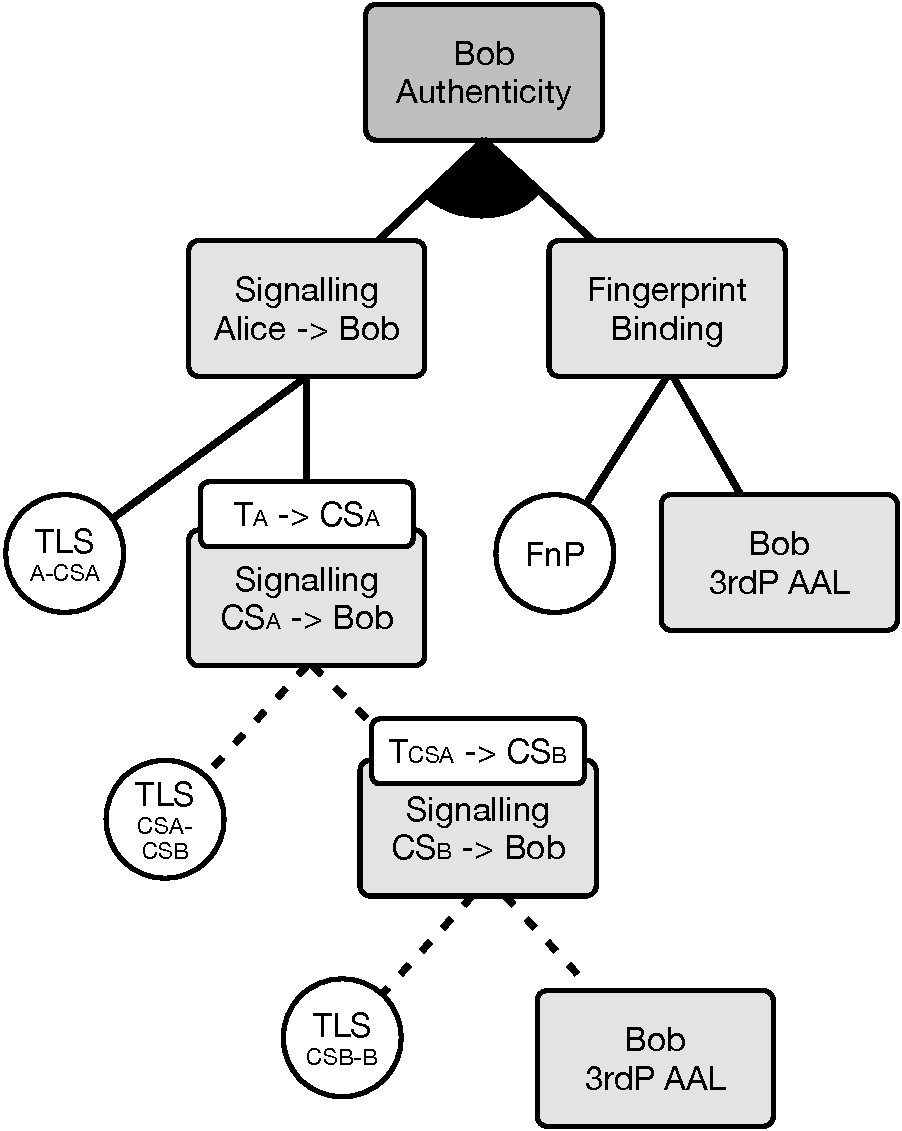
\includegraphics[scale=.5]{images/df_signalling}
\caption{Graphical representation.}
\end{subfigure}
~
\begin{subfigure}[b]{0.4\textwidth}
\begin{equation*}
\begin{split}
&T_A(auth(B)) \quad\oplus \\
&    \quad T_A(sig(A,B)) \quad\otimes \\
&        \quad\quad TLS(A,CS_A) \\
&        \quad\quad T_A(CS_A) \textcolor{matgrey}{\rightarrow} \\
&        \quad\quad \textcolor{matgrey}{T_{CS_A}(sig(CS_A,B)) \quad\otimes}  \\
&            \quad\quad\quad \textcolor{matgrey}{TLS(CS_A, CS_B)} \\
&            \quad\quad\quad \textcolor{matgrey}{T_{CS_A}(CS_B) \rightarrow} \\
&            \quad\quad\quad \textcolor{matgrey}{T_{CS_B}(sig(CS_B,B)) \quad\otimes} \\
&                \quad\quad\quad\quad \textcolor{matgrey}{TLS(CS_B, B)} \\
&                \quad\quad\quad\quad \textcolor{matgrey}{T_{CS_B}(3pAAL(B))} \\
&    \quad T_A(binding(FnP_B,B)) \quad\otimes \\
&        \quad\quad FnP_B \\
&        \quad\quad T_A(3pAAL(B)) \\
\end{split}
\end{equation*}
\caption{Outline form.}
\end{subfigure}
\caption{Alice's trust in Bob's authenticity resulting from the signalling process.}
\label{fig:df_signalling}
\end{figure}

\subsection{Identity Path Security}
As we explain, the WebRTC identity assertion mechanism binds Bob's fingerprint received over the signalling path to an identity assertion issued by Bob's identity provider $IdP_B$.
This assertion is verified by the browser instantiating an \gls{idp} Proxy (see Section~\ref{sec:webrtcidpath}).
The security of this process relies on four dependencies presented in Figure~\ref{fig:df_identity}.

Regarding the verification of the identity assertion, Alice must be able to communicate securely with $IdP_B$.
This includes the download of the \gls{idp} Proxy over \gls{https}, a policy enforced by the WebRTC specification, but also subsequent communications between the \gls{idp} Proxy and the \gls{idp} server.
The verification of the identity assertion must also be secure against integrity attacks.
We note the trust in the identity assertion as $T_A(Tkn_B)$ although the exact nature of the identity assertion depends on the protocol implemented by the \gls{idp}.
For instance, one of our implementation presented in Section~\ref{sec:idpoidc} uses a \gls{jwt} containing the user's fingerprint.
Compromising the integrity of the \gls{jwt} could allow an attacker to impersonate one of the peers and mount a \gls{mitm} attack.

Alice also needs to trust Bob's \gls{idp}, noted $T_A(IdP_B)$, and its authentication of Bob.
However, this process is not visible from Alice.
Nonetheless, we represent it in dashed lines in graphical form and grey font in outline form.
In some cases, the \gls{idp} may recommend Bob's authentication strength, for instance using the \gls{oidc} \gls{acr} claim.
We note this recommendation $T_{IdP_B}(AAL(B))$ which depends on the authentication strength of Bob and the presence of a secure connection between Bob and his \gls{idp}.

\begin{figure}[tb]
\centering
\begin{subfigure}[b]{0.55\textwidth}
\centering
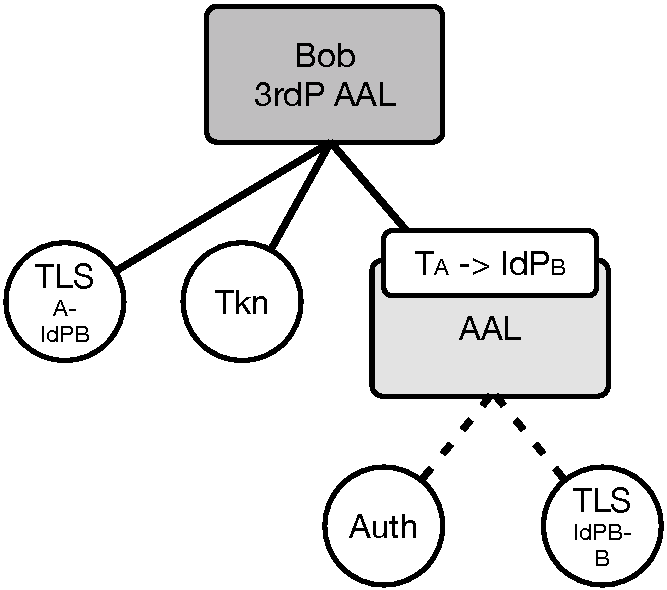
\includegraphics[scale=.5]{images/df_idBinding}
\caption{Graphical representation.}
\end{subfigure}
~
\begin{subfigure}[b]{0.4\textwidth}
\begin{equation*}
\begin{split}
& T_A(3pAAL(B))  \quad\otimes \\
&    \quad TLS(A,IdP_B) \\
&    \quad Tkn_B \\
&    \quad T_A(IdP_B) \rightarrow \\
&    \quad T_{IdP_B}(AAL(B)) \textcolor{matgrey}{\quad\otimes} \\
&         \textcolor{matgrey}{\quad\quad Auth(B)} \\
&         \textcolor{matgrey}{\quad\quad TLS(B,IdP_B)} \\
\end{split}
\end{equation*}
\caption{Outline form.}
\end{subfigure}
\caption{Alice trust in Bob's identity path.}
\label{fig:df_identity}
\end{figure}

Supposing that $CS_B$ authenticated Bob using an authentication delegation protocol, the same decomposition could be applied to the trust of $CS_B$ in Bob's authenticity noted $T_{CS_B}(3pAAL(B))$ and presented in Figure~\ref{fig:df_signalling}.
As we remarked in Section~\ref{sec:webrtcidpath}, in most cases the same \gls{idp} would be used by Bob to authenticate to $CS_B$ and Alice.

\subsection{Media Path Confidentiality}
The confidentiality of the media path is ensured by the \gls{srtp} protocol using \gls{dtls} for handshake and keying and vulnerabilities or weak security level on either of these protocols could lead to a compromised encryption of the media path.
The WebRTC security architecture~\cite{I-D.ietf-rtcweb-security-arch} mandates the implementation of \gls{dtls} 1.0 and recommends the implementation of \gls{dtls} 1.2.
Guidelines regarding the implementation of cypher suites and SRTP profiles are also given. 
%In addition, Bob's fingerprint, noted $FnP_B$, binds his \gls{dtls} key used in the media plane to the signalling plane~\cite{RFC5763}.
%To represent this binding, this fingerprint is included in both the Media Confidentiality and Bob Authenticity sub-tree.
%For instance, implementations must at least offer the following cypher suite: TLS\_ECDHE\_ECDSA\_WITH\_AES\_128\_CBC\_SHA with the P-256 curve.
The trust of Alice in the media path confidentiality thus depends on the strength of the protocols and the cypher suite in use as presented in Figure~\ref{fig:df_media}.


\begin{figure}[tb]
\centering
\begin{subfigure}[b]{0.5\textwidth}
\centering
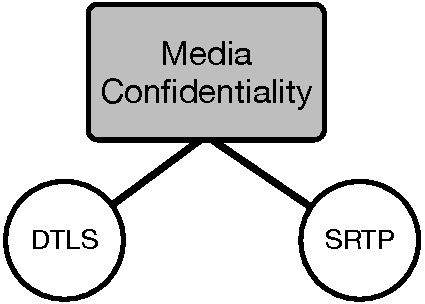
\includegraphics[scale=.5]{images/df_mediaConf}
\caption{Graphical representation.}
\end{subfigure}
~
\begin{subfigure}[b]{0.45\textwidth}
\begin{equation*}
\begin{split}
&T_A(conf(M_{\{A,B\}})) \quad\otimes \\
&    \quad DTLS\\
&    \quad SRTP\\
%&    \quad FnP_B\\
\end{split}
\end{equation*}
\caption{Outline form.}
\end{subfigure}
\caption{Alice's trust in the confidentiality of the peer-to-peer media streams.}
\label{fig:df_media}
\end{figure}

\subsection{Overall Trust and Security Tree, Instantiation and Computational Models}
Combining the previous subtree, we reconstruct the whole trust and security tree as presented in Figure~\ref{fig:dfoverall}.
Leafs of the decomposition tree are either security elements \eg $Tkn_B$, or trust in actors of the communication setup \eg $T_A(IdP_B)$.
In order to instantiate the model, it is necessary to assign values to these leaf elements and a computational model to $\otimes$ and $\oplus$ nodes.
The model can then be evaluated to return an overall value representing the security of the WebRTC session to the user.


\begin{figure}[tb]
\centering
\begin{subfigure}[b]{0.55\textwidth}
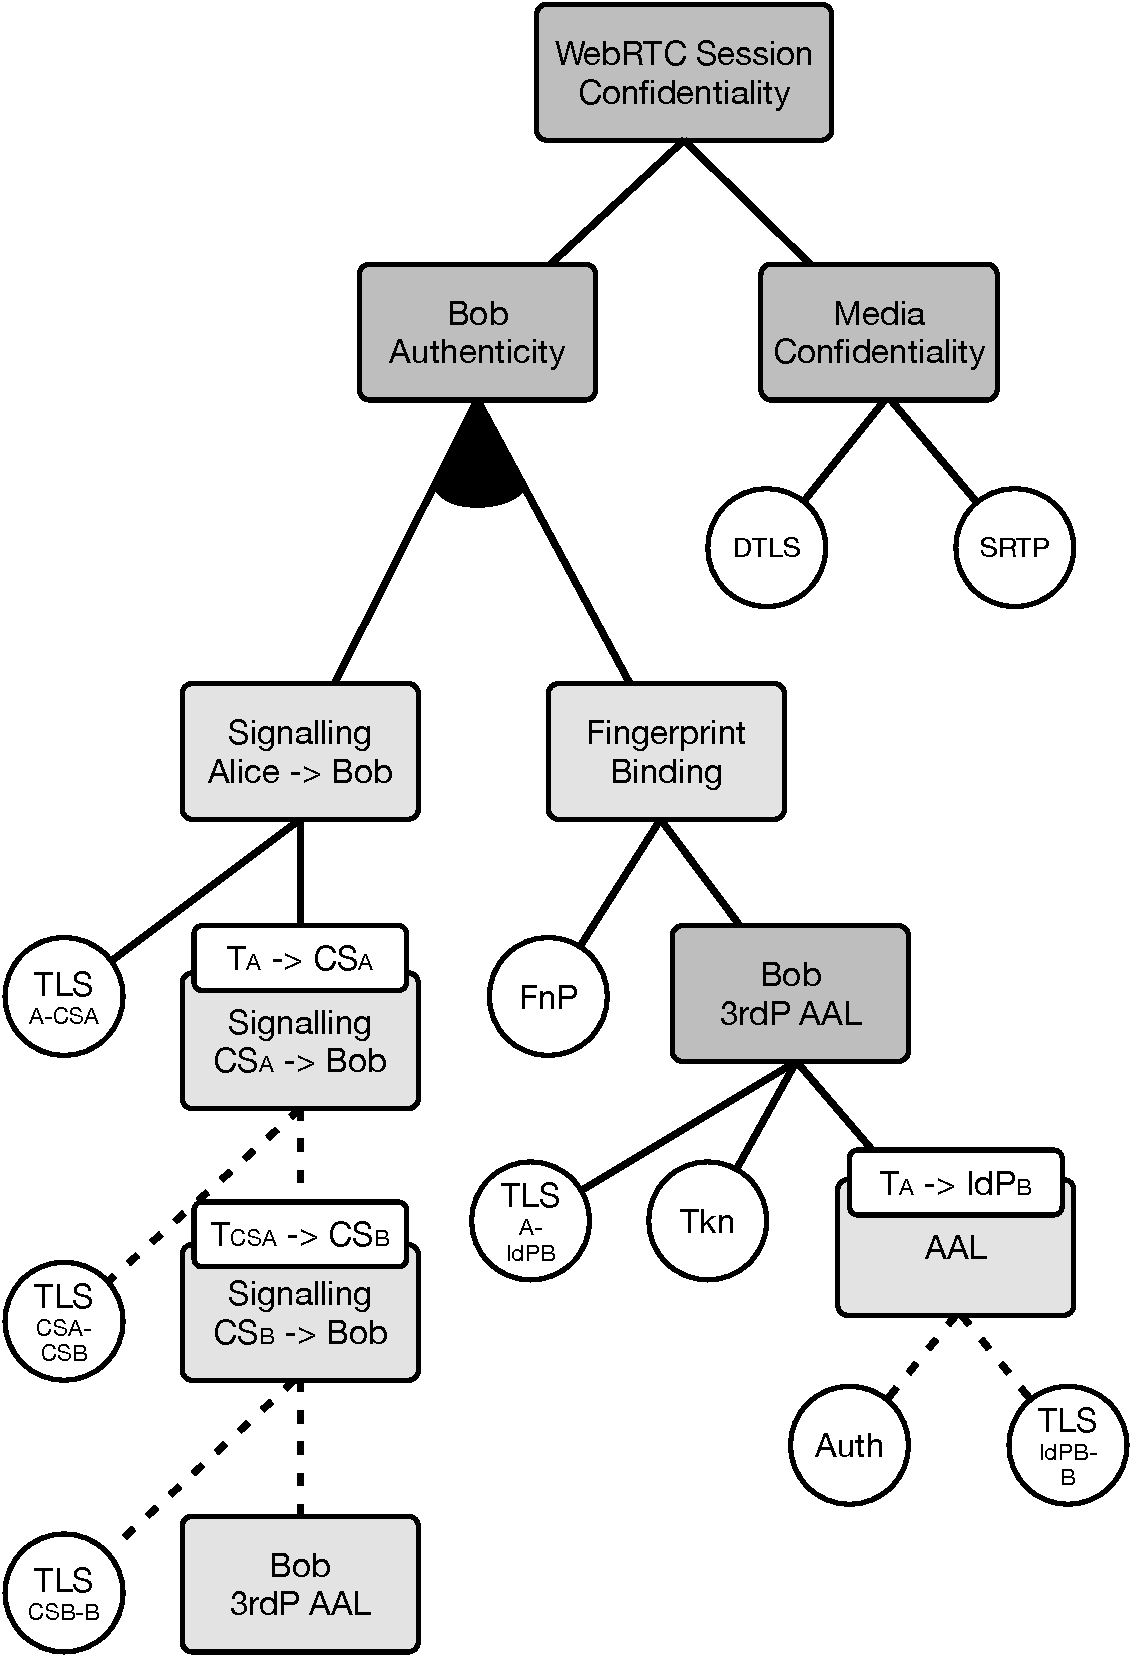
\includegraphics[scale=.4]{images/df_overall}
\caption{Graphical representation.}
\end{subfigure}
~
\begin{subfigure}[b]{0.4\textwidth}
\begin{equation*}
\begin{split}
&T_A(conf(Session_{A,B,M})) \quad\otimes \\ 
&    \quad T_A(auth(B)) \quad\oplus \\ 
&        \quad\quad T_A(sig(A,B)) \quad\otimes \\
&            \quad\quad\quad TLS(A,CS_A) \\
&            \quad\quad\quad T_A(sig(CS_A,B)) \quad\otimes \\
&                \quad\quad\quad\quad T_A(CS_A) \\
&                \textcolor{matgrey}{\quad\quad\quad\quad TLS(CS_A, CS_B)} \\
&                 \textcolor{matgrey}{\quad\quad\quad\quad T_{CS_A}(sig(CS_B,B)) \quad\otimes} \\
&                     \textcolor{matgrey}{\quad\quad\quad\quad\quad T_{CS_A}(CS_B)} \\
&                     \textcolor{matgrey}{\quad\quad\quad\quad\quad TLS(CS_B, B)} \\
&                     \textcolor{matgrey}{\quad\quad\quad\quad\quad T_{CS_B}(3pAAL(B))} \\
&        \quad\quad T_A(binding(FnP_B,B))  \quad\otimes \\
&            \quad\quad\quad FnP_B \\
&            \quad\quad\quad T_A(3pAAL(B)) \quad\otimes \\
&                \quad\quad\quad\quad T_A(IdP_B) \\
&                \quad\quad\quad\quad TLS(A,IdP_B) \\
&                \quad\quad\quad\quad T_A(Tkn_B) \\
&                \quad\quad\quad\quad T_{IdP_B}(AAL(B))  \textcolor{matgrey}{\quad\otimes} \\
&                         \textcolor{matgrey}{\quad\quad\quad\quad\quad auth(B)} \\
&                         \textcolor{matgrey}{\quad\quad\quad\quad\quad TLS(B,IdP_B)} \\
&    \quad T_A(conf(M_{\{A,B\}})) \quad\otimes \\
&        \quad\quad DTLS\\
&        \quad\quad SRTP\\
%&        \quad\quad FnP_B\\
\end{split}
\end{equation*}
\caption{Outline form.}
\end{subfigure}
\caption{Overall trust of Alice in the confidentiality of her WebRTC session.}
\label{fig:dfoverall}
\end{figure}

In Section~\ref{sec:trustintro}, when introducing the concept of trust, we explained that trust models are generally categorised between policy and reputation-based trust.
Supposing the definition of some policy rules, trust in actors could be represented as a boolean.
Users could configure such policies in their browsers for instance as a list of trusted actors.
A similar functionality is already implemented by browsers for the management of web \gls{api} authorization granted to web origins.
Alternatively, trust model can rely on reputation trust, often represented as a continuous score, for instance on $[0;1]$.
This is the approach followed by the many reputation models such as from Javed~\etal\cite{javed2016browser} which suppose either a centralised recommendation source or a distributed reputation model based on users' opinions.
However, managing too many permissions may be difficult for users and their permanent nature may result in vulnerabilities as reported by the STREWS project~\cite{bos2014case}.
The web browser or a third-party could also provide such recommendation lists, for instance in a similar fashion to add-blocking extensions\footnote{Although this model also has its limits as add blockers gain a powerful and somewhat illegitimate position.}.

Regarding values for security elements, we reported in the state of the art (Section~\ref{sota2012}) how national security agencies publish recommendations on security algorithms implementation and usages based on prior work by Lenstra~\cite{Lenstra2004}.
As with trust, policies can define good enough security level, for instance, based on implemented cypher suites and \gls{aal}.
While compliance with such policies can be represented as boolean values an alternative is to use numerical values. 
For instance, Alia \etal\cite{alia2010putting} use such values for their security utility functions, although apparently arbitrarily defined.
In order to derive numerical values for a security utility function, a solution is to divide the implemented key length by the recommended key length bounded to one:

\begin{figure}[H]
\begin{equation*}
F(k,r) = \left\{
    \begin{array}{ll}
        2^{k-r} & \mbox{if } k \leq r \\
        1 & \mbox{else.}
    \end{array}
\right.
\end{equation*}
\caption[Comparative Security Utility Function]{Comparative security utility function with $k$ the actual key size and $r$ the recommended key size both expressed in bits.}
\end{figure}

Table~\ref{tab:ownUtilityFunction} gives an example instantiation of such function over a WebRTC setup.
In this example, Alice uses the Chrome web browser to visit a WebRTC website and connect to Bob.
The website $CS_A$ provides a ``Let's encrypt certificate'' and the connection is encrypted using the AES symmetric encryption algorithm.
The ANSSI recommends a 100 bits key size for symmetric encryption algorithms~\cite{ANSSI} and in this instance, a 256 bits key is used.
\gls{dtls} and \gls{srtp} are then used to establish the WebRTC session.
More particularly, only the \gls{dtls} ECDHE key exchange and the ECDSA authentication mechanism are used with the P-256 curve, meeting the recommended key size for elliptic curves.
The certificate's fingerprint is a SHA256 hash which also meets the recommendations.
Once the connection is established Alice asks Bob to authenticate using the solution described in Section~\ref{sec_sdp}.
The \gls{tls} session between Alice and $IdP_B$ uses the same configuration as for $CS_A$.
Finally, the identity assertion is a \gls{jwt} signed with the RS256, \ie RSASSA-PKCS1-v1\_5 using SHA256 which also meets the recommendations.

\begin{table}[tb]
\begin{tabular}{{@{}p{6cm}cccc@{}}}\toprule\toprule
Security Element & Key Length & Category (rec) & Value \\\midrule
\small{$TLS$~~~~$A-CS_A / A-IdP_B$} \newline \tiny{TLS\_ECDHE\_RSA\_WITH\_AES\_256\_GCM\_SHA384} & 256 & Sym (100) & 1 \\

\small{$DTLS$} \newline \tiny{TLS\_ECDHE\_ECDSA\_WITH\_AES\_128\_GCM\_SHA256} & P-256 & EC (200) & 1 \\

\small{$SRTP$} \newline \tiny{AES\_CM\_128\_HMAC\_SHA1\_32} & 128 & Sym (100) & 1 \\

\small{$FnP_B$} \newline \tiny{SHA256} & 256 & Hash (200) & 1 \\

\small{$Tkn_B$} \newline \tiny{RSASSA-PKCS1-v1\_5 using SHA256} & 256 & Hash (200) & 1\\

  \bottomrule
  \hline
\end{tabular}
\caption{Security element instantiation based on ANSSI recommendations~\cite{ANSSI}.}
\label{tab:ownUtilityFunction}
\end{table}

The operator $\otimes$ represents weakest link dependencies, \ie all trust or security dependencies must hold for the parent property to hold. 
The value of an $\otimes$ node is thus the minimum value of each of its dependencies.
Symmetrically, the operator $\oplus$ represents situations where at least one dependency must hold for the parent property to hold.
We thus define the value of an $\oplus$ node as the maximum value of each of its dependencies.
These two operators allow us to represent the trust and security view from the user's point of view, \ie limited to what the browser can monitor.
However, we also extended our trust and security tree to relations between other actors, \eg Bob's authentication by his \gls{idp} in Figure~\ref{fig:df_identity}.
These extensions are characterised by transitive trust relations, \eg Alice's trust in Bob's \gls{idp} in Figure~\ref{fig:df_identity}.
To evaluate such transitive trust, we use the trust relationship as a weight to its dependency value.
Figure~\ref{def:df_overall} presents the overall formula for evaluating the trust of Alice from both her point of view and from an omniscient point of view.
 
\begin{figure}[tb]
\centering
\begin{subfigure}[b]{0.47\textwidth}
\begin{equation*}
\begin{split}
&T_A(Session_{A,B,M}) = \\
&MIN(\\
&\quad MAX(\\
    &\quad\quad MIN(\\
        &\quad\quad\quad TLS(A,CS_A),\\
        &\quad\quad\quad T_A(CS_A) \\
    &\quad\quad ),\\
    &\quad\quad MIN(\\
        &\quad\quad\quad FnP_B,\\
        &\quad\quad\quad TLS(A,IdP_B),\\
        &\quad\quad\quad Tkn_B,\\
        &\quad\quad\quad T_A(IdP_B)\\
&\quad )),\\
&\quad DTLS,\\
&\quad SRTP\\
&)
\end{split}
\end{equation*}
\caption{Alice's point of view.}
\end{subfigure}
~
\begin{subfigure}[b]{0.47\textwidth}
\begin{equation*}
\begin{split}
&T_A(Session_{A,B,M}) = \\
&MIN(\\
&\quad MAX(\\
    &\quad\quad MIN(\\
        &\quad\quad\quad TLS(A,CS_A),\\
        &\quad\quad\quad T_A(CS_A) * MIN(\\
            &\quad\quad\quad\quad TLS(CS_A, CS_B),\\
            &\quad\quad\quad\quad T_{CS_A}(CS_B) * MIN(\\
                &\quad\quad\quad\quad\quad TLS(CS_B, B),\\
                &\quad\quad\quad\quad\quad T_{CS_B}(IdP_B)*MIN(\\
                &\quad\quad\quad\quad\quad\quad  Auth(B),\\
                &\quad\quad\quad\quad\quad\quad  TLS(B,IdP_B))))\\
    &\quad\quad ),\\
    &\quad\quad MIN(\\
        &\quad\quad\quad FnP_B,\\
        &\quad\quad\quad TLS(A,IdP_B),\\
        &\quad\quad\quad Tkn_B,\\
        &\quad\quad\quad T_A(IdP_B) * MIN(\\
            &\quad\quad\quad\quad AAL(B),\\
            &\quad\quad\quad\quad TLS(B,IdP_B))\\
&\quad )),\\
&\quad DTLS,\\
&\quad SRTP\\
&)
\end{split}
\end{equation*}
\caption{Omniscient point of view.}
\end{subfigure}

\caption{Overall computational formula for Alice trust in her WebRTC session.}
\label{def:df_overall}
\end{figure}


\section{Validation}
\label{sec:validationModel}

Our WebRTC trust and security model is designed to help end-users understand the security of their communications and how their trust in actors of their WebRTC setup may influence their security.
Similarly to the secure connection indications implemented by web browser, \ie the \gls{https} green lock, our model can be instantiated and evaluated to return a single value.
It could also be presented in an instantiated graphical form to provide a detailed view of the situation intended for advanced users, again similarly as to how web browser display details on \gls{https} certificates.
While the usage of a coloured icon as a way to provide a security indicator is already deployed in browser, this is not the case of our trust and security decomposition model.
In this section, we intend to answer the following questions:
\begin{itemize}
\item \textbf{RQ1.2} How do users understand the definition of trust in actors of the communication setup?
\item \textbf{RQ1.3} Does our trust and security model helps users understand the security of their WebRTC communication?
\end{itemize}

\subsection{WebRTC Trust and Security Model Survey}

To this end, we conducted an online survey that we distributed to researchers in our team.
Compared to a more generic end-user population, we believe that this population is more concerned with the security of their communications and as such more susceptible to search for a detailed view of a communication security setup.
However, compared to security experts, communication security is not an area of focus for our research team.
We thus estimate that this population corresponds to the category of end-users that would like to understand what's happening ``behind the hood'' but may need the help of an high-level model to grasp the situation.
As the size of the surveyed population is however quite limited, we do not claim any representativity of our results but we see them as preliminary.
More investigations may be needed.

One of the design goals of our survey is that we want participants to express their own intuitive understanding of the trust and security setup helped by our model. 
The difficulty lies in how we explain our model and WebRTC security, without influencing too much the participants.
For instance, giving a crash course on WebRTC basically saying ``WebRTC is secure if a third-party \gls{idp} is used'' would help participants understand the WebRTC security architecture, but it would not reveal if this understanding was due to our model or not.
Throughout the survey, we thus walk a narrow line where we provide a limited description of the \gls{voip} or WebRTC scenarios and architectures.

The survey is organised in four successive page\footnote{The survey is accessible at \url{http://kcorre.github.io/webrtcsurvey}.}.
On the first page, we recall how web browser asserts the confidentiality and authenticity of \gls{https} connection to website by displaying a green lock icon.
We then briefly explain our objective and that the survey will be used to evaluate the interest, usefulness, and clarity of our security model.
The intended duration of the survey, ten minutes, is also stated.
The last page is used to let participants qualify their expertise in the fields of web technologies, computer security, and real-time communication technologies.
For each field of expertise, participants are instructed to choose an expertise level between end-user, intermediate, and expert. 
The bulk of the survey's questions are on page two and three which we detail below. 

In the second page, the survey focuses on trust in audio and video communications.
We first present the role of \gls{cs} in \gls{voip} services and their responsibility of the signalling and authentication of participants.
After defining WebRTC illustrated with a basic WebRTC architecture, we explain how identity providers allow users to authenticate by exchanging identity assertions.
We then define several real-time communication scenarios and request participants to evaluate their trust in such scenarios regarding the confidentiality of their communications.
We propose a trust scale between 0 and 10 in the context of communication confidentiality and privacy, defined as follows:
\begin{quote}\textit{``On this scale, 10 represents an absolute trust that actors in the communications setup or external attackers are not breaching, or are not able to breach, the confidentiality and privacy of your communication. While 0 stands for a total distrust. i.e. an attack could be mounted as with a weak security level.''}
\end{quote}
Formulated as such, trust is a subjective measure.
Our intent here is both to exemplify various real-time communication deployments and to see if users feel comfortable in attributing trust score to \gls{voip} scenarios and their underlying communication services.
The scenarios described in our survey are: 
\begin{itemize}
\item A national mobile phone call.
\item An international mobile phone call.
\item A well-known web communication service, \eg Skype, Messenger, or Whatsapp.
\item A web meeting service provided by your company.
\item A web service for hosting work meeting and discussions, \eg Slack, Fleep, Appear.in.
\item A WebRTC enabled webpage providing a call widget to a customer service; \eg a banking website.
\item An untrusted WebRTC communication service with a third-party identity assertion from a known identity.
\item A Real-Time Communication service using an old plugin and unspecified security parameters, \eg with a Flash plugin.
\end{itemize}

Basically, these scenarios describe three communication service categories: legacy phone services, web \gls{ott} services, and ubiquitous WebRTC services.
Comparisons can be drawn between scores attributed to scenarios in the same categories and between categories.
In scenarios describing mobile phone services, we insist on the difference between national and international call.
As we explained previously, the telco model relies on trust circles to integrate multiples operators. 
While telco operators are not explicitly visible when receiving a call, national operators are at least known to the users which may less be the case for international operators. 
In scenarios describing web \gls{ott} services, we insist on three categories of services: big \gls{ott} player often feared and criticised for their dominant position, smaller communication services which may benefit from a better image, and services officially recommended or provided by the user's company.
These scenarios are thus intended to reveal trust based on subjective opinion rather than technical setup.
In the WebRTC service category, we intend to see how users may intuitively trust the WebRTC identity architecture.
The WebRTC enabled webpage scenario is exemplified with a banking website which should suggest high-security standards and thus trust.
On the contrary, in the second WebRTC scenario, we specifically describe an untrusted WebRTC \gls{cs}, although backed by a trusted \gls{idp}.
In the WebRTC security architecture~\cite{I-D.ietf-rtcweb-security-arch}, such scenario is used to justify the use of the third party \gls{idp}. 
Finally, the last scenario suggests a service using a weak security level or with existing vulnerabilities.

\begin{figure*}[p]
\centering
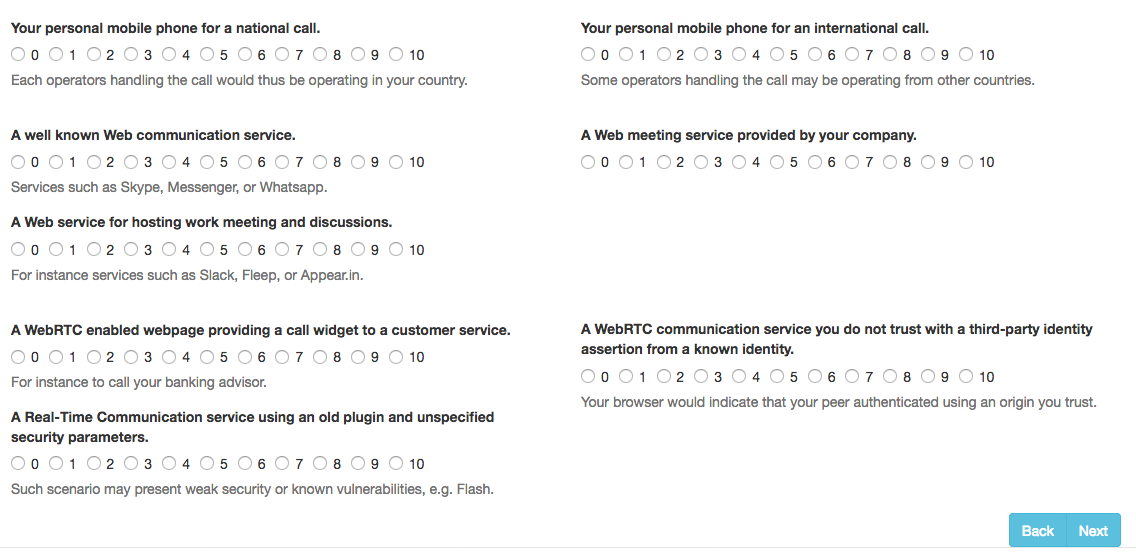
\includegraphics[scale=.55,angle=90]{images/surveyTrust}
\caption{Survey: Trust in Communication Scenarios.}
\label{fig:surveyTrust}
\end{figure*}

\begin{table}
\begin{tabular}{{@{}lccccccccccc@{}}}\toprule\toprule
 Scenario & u1 & u2 & u3 & u4 & u5 & u6 & u7 & u8 & u9 & u10 & Mean\\\midrule
 Mobile  & 3 & 6 & 9 & 9 & 3 & 6 & 6 & 7 & 7 & 0 & 5.6 \\
 Int. Mobile & 2 & 4 & 7 & 4 & 3 & 5 & 5 & 4 & 6 & 0 & 4 \\\midrule
 Big OTT & 3 & 6 & 6 & 6 & 3 & 6 & 6 & 6 & 7 & 3 & 5.2 \\
 Small OTT & 3 & 6 & 4 & 6 & 4 & 8 & 8 & 5 & 4 & 3 & 5.1\\
 Company & 4 & 6 & 6 & 7 & 3 & 9 & 8 & 8 & 8 & 0 & 5.9 \\\midrule
 WebRTC & 3 & 3 & 3 & 5 & 5 & 8 & 8 & 5 & 2 & 3 & 4.5 \\
 WebRTC IdP & 2 & 1 & 5 & 6 & 3 & 6 & 0 & 5 & 1 & 3 & 3.2 \\\midrule
 Insecure & 1 & 2 & 0 & 3 & 3 & 0 & 0 & 0 & 0 & 0 & 0.9 \\\midrule
 Trust scale & 1-4 & 1-6 & 0-9 & 3-9 & 3-5 & 0-8 & 0-8 & 0-8 & 0-8 & 0-3 & -\\
  \bottomrule
  \hline
\end{tabular}
\caption[Survey results: Trust in Audio and Video Communications]{Survey results: trust in audio and video communications.}
\label{tab:surveyTrust}
\end{table}

Submitted results are presented in Table~\ref{tab:surveyTrust}.
As the surveyed population is not representative we do not draw any conclusions but bring some remarks to the reader's attention.
We expected attributing trust values to be a clearly subjective task. 
However, as we observe that trust values in a given scenario are quite different for each participant, we also observe that participants use different trust scales.
This may reveal that a single trust value may not have the same meaning for two users.
We also note that each participant who rated the insecure scenario with a trust value superior to 0 also qualified their experience with computer security as ''end-users''.
Another interesting observation is the mean trust of the WebRTC \gls{idp} scenario.
With the exception of the insecure scenario, the WebRTC \gls{idp} scenario has the lowest mean trust.
Further investigation may thus show that providing an identity assertion may not be enough for users to trust any WebRTC enabled website.

In the third page of the survey, we let participants play with a dynamic implementation of our trust and security model in graphical form as presented in Figure~\ref{fig:d3Model}.
The model represents high-level trust property as coloured nodes depending on their actual trust values, and security properties as small black nodes.
A panel in the top-left corner let participants define various trust relations.
Similarly, a list of radio button elements corresponding to communication scenarios on the previous page let participants select trust configurations.
In this mode, the actual trust values depend on the trust values previously defined by the participant.
For instance, if one participant set a trust value of 6 to the WebRTC \gls{idp} scenario, selecting this scenario on the dynamic trust model would set the following trust relations: $T_A(CSA) =0$ and $T_A(IdP_B)=0.6$.
Participants can also interact with black security nodes by double-clicking on them in order to modify the nodes' value.
In order to explain the model, a limited description of the modelled WebRTC scenario is provided as reproduced in Figure~\ref{fig:modelExplanation}.
The dynamic model also displays tip note when hovering over high-level and security nodes, mainly used to explain acronyms.

%\begin{figure*}[H]
%\begin{subfigure}[b]{0.55\textwidth}
%\begin{quote}
%\textit{``Here we model the security and trust of a WebRTC session. The idea is to represent the trust that a user may have in the confidentiality of his communication. We consider a call-session involving two participants, \textbf{Alice (you) and Bob}. Each participants use a different communication service, \textbf{CSA} and \textbf{CSB}.}
%
%\textit{Bob also provides an identity assertion signed by and verified through \textbf{IdPB}, his Identity Provider. This identity assertion binds the fingerprint of the session, \textbf{FnP}, to Bob's identity ensuring that no one is able to impersonate Bob.''}
%\end{quote}
%\end{subfigure}
%~
%\begin{subfigure}[b]{0.45\textwidth}
%\centering
%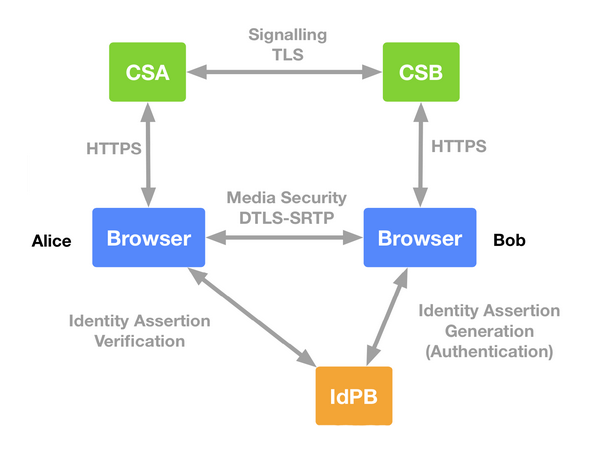
\includegraphics[scale=.65]{images/webrtcExplanation}
%\caption[WebRTC Scenario of the Dynamic Trust and Security Model]{Description of the WebRTC scenario represented by the dynamic trust and security model.}
%\label{fig:modelExplanation}
%\end{subfigure}
%\end{figure*}

\begin{figure*}[p]
\centering
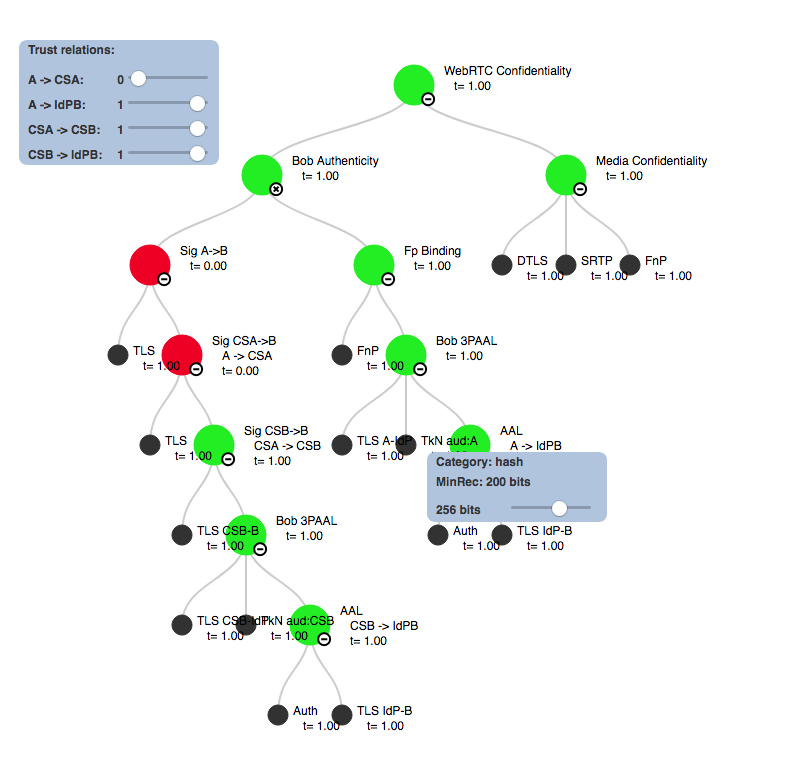
\includegraphics[scale=.65]{images/webrtcD3Model}
\caption{WebRTC Trust and Security Model implementation in D3.js.}
\label{fig:d3Model}
\end{figure*}

\begin{figure*}[p]
\centering
\begin{subfigure}[b]{0.45\textwidth}
\centering
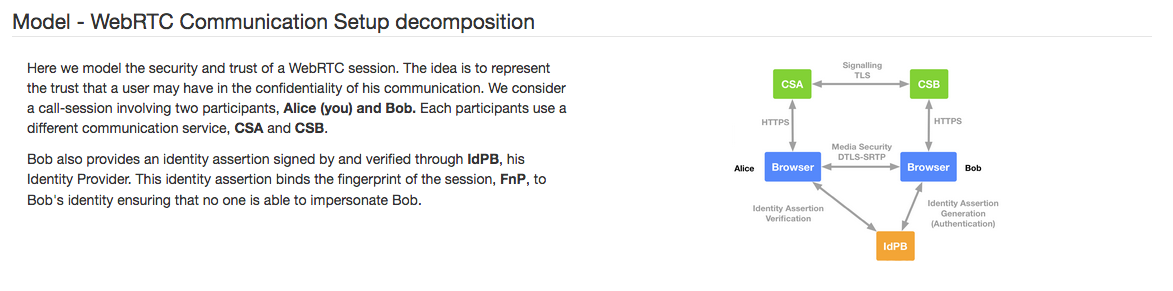
\includegraphics[scale=.5,angle=90]{images/surveyDescr}
\caption{Description of the WebRTC scenario of the dynamic model.}
\label{fig:modelExplanation}
\end{subfigure}
\begin{subfigure}[b]{0.55\textwidth}
\centering
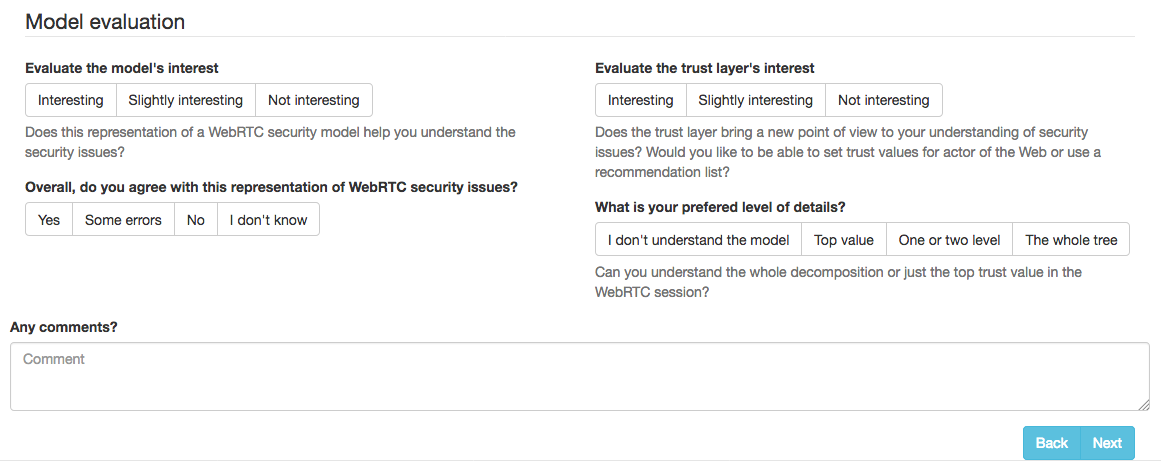
\includegraphics[scale=.5,angle=90]{images/surveyInterest}
\caption{Survey Questions}
\label{fig:surveyInterest}
\end{subfigure}
\caption{Survey: Interest in the WebRTC Trust and Security Model.}
\end{figure*}

Finally, participants are invited to evaluate their interest for the presented WebRTC security model and the trust layer, as in Figure~\ref{fig:surveyInterest}. 
The proposed values for both questions are \textit{Interesting},  \textit{Slightly interesting}, and \textit{Not interesting}.
Participants are also instructed to state up to which decomposition level are they able to understand the model.
The proposed values are \textit{I don't understand the model}, \textit{Top value}, \textit{One or two level}, and \textit{The whole tree}.
The survey also offers a text box for comments and we gathered other feedbacks in face to face discussions.
Results of this part of the survey are presented in Table~\ref{tab:surveyInterest}.


\begin{table}[tb]
\begin{tabular}{{@{}lcccccccccc@{}}}\toprule\toprule
 Interest & u1 & u2 & u3 & u4 & u5 & u6 & u7 & u8 & u9 & u10 \\\midrule
 WebRTC model & 2 & 2 & 1 & 1 & 2 & 2 & 2 & 1 & 2 & 2 \\
 Trust layer & 2 & 2 & 1 & 1 & 1 & 2 & 2 & 1 & 2 & 2 \\\midrule
 Detail level & Some & Some & Top & Some & Some & All & All & Top & All & Some\\ 
  \bottomrule
  \hline
\end{tabular}
\caption[Survey results: Interest of the Trust and Security Model]{Survey results: Interest of the trust and security model. Interest for the WebRTC model and trust layer correspond to \textit{Interesting} (2),  \textit{Slightly interesting} (1), and \textit{Not interesting}(0). On the detail level line, \textit{Top} stands for only the top value, \textit{Some} stands for only one or two decomposition level, and \textit{All} stands for the whole model}.
\label{tab:surveyInterest}
\end{table}

Again, our results are not representative and we limit ourselves to observations.
Although the survey is anonymous, rating the interest of the model in such manner probably gives biased results probably.
It is thus more interesting to look at the evaluation of the interest in conjunction with the level of decomposition the participants were able to understand the model.
Three answerers \textit{-u6, u7, u9-} declared that they understood the whole model and that it is an interesting representation of WebRTC security and trust relations.
None of these declared themselves an expert in any categories. 
Other participants \textit{-u1, u2, u5, u10-} found an interest in the model but did not understand the whole decomposition declared.
Finally, some participants \textit{-u3, u8-} only understood the top value and only found a slight interest in the model \textit{-u3, u4, u8-}.
The comments and discussions also indicated that the meaning of lower decomposition levels where difficult to understand and not adapted for end-users.
Even with the help of tip notes to explain nodes.
It is also interesting to see that participants who declared to understand the whole tree \textit{-u6, u7, u9-} did not rate themselves as web technologies experts on the contrary to some participants who did not understand the whole model \textit{-u1, u2, u5, u10-}.
As a participant reported ``the model [...] is interesting for people who do not have much knowledge in the field but still are interested in knowing how it roughly works.''
On the other hand, it may not be satisfying for people with more experience in web technologies who would have higher expectations before declaring themselves able to understand the model.


\subsection{Discussions}
\label{sec:webrtcmodelDiscuss}
As we explain, the validation of our WebRTC trust and security model is limited to a preliminary experiment.
In the future, we intend to conduct further investigation on a larger population. 
Evaluating trust in a survey's artificial setting is a complex and difficult task. 
Nevertheless, the preliminary study helped in identifying avenues for refinement.
 
In the survey, we explicitly instructed participants to consider trust in the context of the confidentiality and privacy of their communications.
However, some participants reported a difficulty to contextualise this trust without visible communication scenario.
We envision that rather than explaining the WebRTC architecture, our large-scale survey should include an instance of a WebRTC communication service.
This communication service would give a sense of context for the model and its trust and security parameters to the participants.
Similarly, the expression of context in the model is limited to some high-level trust nodes.
In Section~\ref{sec:trustintro} we explained that a trust relation depends on a specific context and that recommendations may allow transitivity from one trust context to others.
A more explicit representation of trust context and context transitivity may help in understanding the model. 
We thus intend to explore how a coloured trust tree could be used to explicitly represent trust context in the model.
We also observe a variation in the numerical trust scales used by users. 
While this variation may be due to different perception of trust for a single scenario, it may also reveal that users do not agree on the meaning of numerical trust values. 
Although our model uses a numerical representation of trust, it may be preferable to let users define trust using natural language. 
This questions the practicality of trust value provided by reputation systems; as a single trust value may not have the same meaning across the whole user population.
This may be worth exploring in future research.

In the survey, and in particular on dynamic model, we represented the whole decomposition tree including transitive relations.
From the interest and understanding scores, we observe that different level of details caters to the expectations of three categories of users. 
In the perspective of a larger scale study, a functionality to let users expand the decomposition tree will be implemented. 
This would let participants select their preferred level of details and focus on what they are able to understand. 
The dynamic model also reveals that in practice, the confidentiality utility function presented in Table~\ref{tab:ownUtilityFunction} is equivalent to a boolean policy.
Indeed, slight change in key size results in large decrease in the security value.
Moreover, cypher suites key size implementations generally vary by more than a few bits.
Instantiating the model's security properties using WebRTC security statistics seems a more practical approach.
Building the survey and the dynamic model around an actual WebRTC communication service will help the implementation of this approach.
However, this requires access to those security statistics provided by browser. 
At the time of writing, Firefox does not publish security statistics for WebRTC session\footnote{\url{about:webrtc}}.
On Chrome, these statistics are accessible from the browser WebRTC statistics\footnote{\url{chrome://webrtc-internals/}} but not from JavaScript code as in Figure~\ref{fig:WebRTCStats}.

\begin{figure}[H]
\begin{Verbatim}[commandchars=\\\{\}]
var \textcolor{matred}{pc} = new RTCPeerConnection()
    [...]
    \textcolor{matred}{pc}.\textcolor{matblue}{getStats}()
    .\textcolor{matblue}{then}(stats => \{
        stats.\textcolor{matblue}{forEach}(stat => \{
            if(stat.type == 'transport')
            console.log(stat)
        \})
    \})
\end{Verbatim}
\caption{This JavaScript code prints \texttt{RTCTransportStats}. However, on Firefox it returns no element, and on Chrome the returned stat does not include \texttt{dtlsCipher} or \texttt{srtpCipher} elements.}
\label{fig:WebRTCStats}
\end{figure}

%\todo{Attention � l'adaptation dynamique, est-ce que c'est notre objectif ou une discussion pour plus tard}

Finally, we remark that Alice's \gls{idp} does not appear in the trust and security model, neither from Alice's point of view or from an omniscient point of view.
On an untrusted \gls{cs}, Alice's \gls{idp} may be the only actor in the communication setup trusted by Alice.
This is paradoxical but easy to explain: as Alice authenticates with her \gls{idp}, for all she knows she may be authenticating to a \gls{mitm} attacker.
It is Bob's \gls{idp} that proves to Alice that the communication is secure.
For this reason, it is important that Alice trusts Bob's \gls{idp}, for instance through a negotiation process as we presented in Section~\ref{sec_sdp}.
An alternative solution could be to use a confirmation mechanism so that Alice's \gls{idp} may be enough for Alice to trust the session.
Such mechanism could draw from ZRTP (see Section~\ref{sec:keymanagement}) or simply be a modification of the existing WebRTC identity validation protocol.

\clearpage

\invisiblesection{Summary}
\label{sec:c3Summary}
%\vspace*{2cm}

\blockmargin%
%\hspace{-\marginparwidth}\hspace{-\marginparsep}
\makebox[\overflowingheadlen][l]{
\begin{minipage}{\overflowingheadlen}

\begin{mdframed}[style=C3Frame,frametitle={Summary}]

In our previous contributions, we have implemented the WebRTC identity architecture and proposed solutions for users to have more control over the WebRTC identity parameters.
We believe that for users to understand, and trust, the security of their communications, they should have more information about the security of their communications.
Web browsers are currently pushing for a secure web and are educating users to look for website security configurations.
However, the security of WebRTC is more difficult to understand as it involves more actors than a simple client-server connection.
In this chapter, we have proposed a model representing the security of a WebRTC session.

\medskip

We presented our methodology based on an iterative decomposition process.
Our model uses the security parameters of the signalling process, media encryption, but also trust parameters configured by the user.
It is a representation of the user's trust in the confidentiality of its session, from its own point-of-view.
However, we also consider the transitive nature of trust relations and propose an omniscient view of the session confidentiality model.
We then discuss an instantiation of our model and propose a utility function for security parameters.

\medskip

To validate our model, we conducted a preliminary experiment on non-experts users.
In this study, we evaluated how users understand the definition of trust in actors of the communication setup and how our trust model helps them understand the security of their WebRTC communication. 
This study was based on an online survey offering participants to interact with a dynamic implementation our model.
This survey helped identify potential difficulties for the understanding of the model and the measure of users perception.

\end{mdframed}

\end{minipage}
}
\unblockmargin